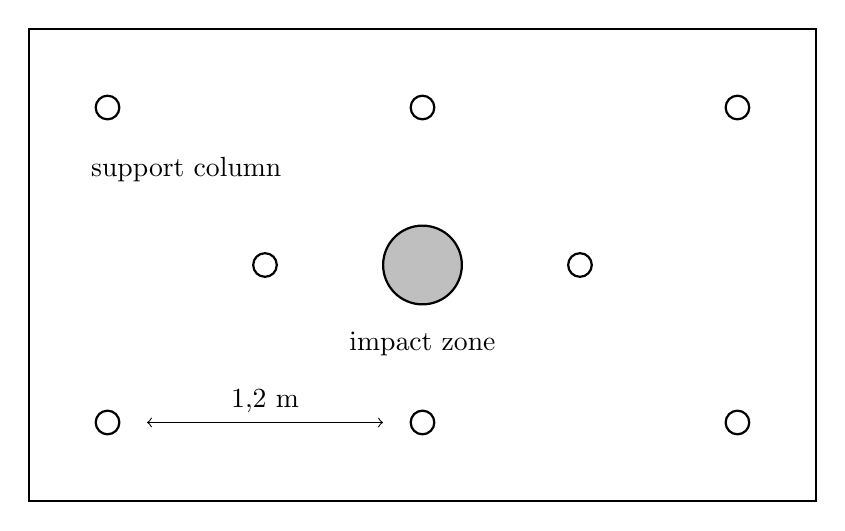
\begin{tikzpicture}
% canadian rock burst drop rig 


\draw[thick] (0,0) -- (10,0) -- (10,6) -- (0,6) -- cycle;
\draw[thick] (1,1) circle [radius=0.15] % pressure points
(5,1) circle [radius=0.15] 
(9,1) circle [radius=0.15] 
(3,3) circle [radius=0.15] 
(7,3) circle [radius=0.15] 
(1,5) circle [radius=0.15] 
(2,4.5) node[align=left, below] {support column}
(5,5) circle [radius=0.15] 
(9,5) circle [radius=0.15];
%[thick] (4.5,2.5)  rectangle (5.5,3.5)
\draw[thick, fill=lightgray] (5,3) circle [radius=0.5];
\draw (5,2) node[align=center] {impact zone}
(3,1) node[align=center,above] {1,2 m};
\draw [<->] (1.5,1) --+ (3,0);
\end{tikzpicture}
